\begin{frame}
	\frametitle{Lecture III Outline}
	\begin{tcolorbox}[coltitle=yellow!50!black,colframe=magenta!25,split=.2,title=Rigid Body Motions]
		Screws and Rigid Body Transformations.
		\tcblower
		Rigid body motions:Properties; Direction cosines; Rotation compositions.
		\vspace{.2cm}
		\newline
		Screws (properly revisited): Chasles' and Poinsot's theorem.
		\vspace{.2cm}
		\newline
		Displacement and Force screws; Pl{\"u}cker coordinates; Homogeneous coordinates;
		\vspace{.2cm}
		\newline
		Rodrigues' formula; the matrix exponential.
	\end{tcolorbox}
\end{frame}

\begin{frame}
	\frametitle{Lecture III Outline}
	\begin{tcolorbox}[coltitle=yellow!50!black,colframe=magenta!25,split=.2,title=Rigid Body Motions]
		Screws and Rigid Body Transformations.
		\tcblower
		Group theory: The Lie algebra, motions in $\mathfrak{se}(3)$;, and the Lie Group.
		\vspace{.2cm}
		\newline
		Transformations: Translations and rotations in $\mathbb{R}^3$, planar rotations, $SO(3), SE(3)$ motions;  homogeneous transformations; Euler and Fick angles; Brockett's exponential map formula. Paden-Kahan subproblems.
	\end{tcolorbox}
\end{frame}

\begin{frame}
	\frametitle{Rigid Body Motions}
	%
	\begin{block}{Rigid Body Motion -- Intro}
		A mapping $g:  \mathbb{R}^3  \rightarrow \mathbb{R}^3$ is a \textcolor{red}{rigid body motion} if 
		\begin{align}
			\|g({x}) - g({y})\| &= \|{x} - {y}\| \text{ for all }  {x}, {y} \in \mathbb{R}^3;  \\
			g({x} \times {y}) &= g(x) \times g({y})\text{ for all }  {x}, {y} \in \mathbb{R}^3; 
		\end{align}
	\end{block}	
	%
	\begin{block}{Rigid Body Motion Preserves Inner Products}
		For two vectors $\bm{a}$ and $\bm{b}$,  $\langle \bm{a},  \bm{b}\rangle =  g(\bm{a}) \times  g(\bm{b})$.
	\end{block}
\end{frame}

\begin{frame}
	\frametitle{Rigid Body Motions as Screws}
	%
	\begin{block}{Rigid Body Motion as a Screw Motion}
		The motion of a \textcolor{red}{rigid body} is precisely the same as if it were attached to  the \textcolor{red}{nut of a literal mechanical screw}. Associated with the screw is its pitch.
	\end{block}	
	%
	\begin{definition}[Screw]
		That straight line with which a \textcolor{red}{definite linear magnitude} termed the pitch is associated is called the \textcolor{red}{screw}.
	\end{definition}
\end{frame}


\begin{frame}
	\frametitle{Screw as a Geometric Quantity}	
	%	
	\begin{block}{Pitch of a Screw}
		\textcolor{brown}{The rectilinear distance}  through which (a literal nut)  \textcolor{red}{nut is translated parallel to the axis of a screw}, while the nut is rotated through the \textcolor{cyan}{angular unit of circular measure} is termed the \textcolor{light-blue}{pitch}.
	\end{block}
	%
	\begin{block}{Pl{\"u}cker Coordinates}
		Let \textcolor{red}{$\bm{a}$} be a point on line $\bm{\ell}_0$. Let \textcolor{red}{$\bm{a}$}'s direction cosine vector (to be introduced shortly) be \textcolor{red}{$\bm{b}$}. Then, its binormal (moment) vector is \textcolor{red}{$\bm{c=a\times b}$}. We say the pair \textcolor{red}{$(\bm{b},\bm{c})$} is the \textcolor{blue}{Pl{\"u}cker Coordinates} of point  \textcolor{red}{$\bm{a}$ on axis} $\bm{\ell}_0$.
	\end{block}	
\end{frame}

\begin{frame}
	\frametitle{Screw in Pl{\"u}cker Coordinates}
	%
	\begin{columns}[b]
		\begin{column}{.67\columnwidth}
			\centering
			\begin{definition}[Screw Coordinates]
				Six-vector, $\bm{s}$, related to the Pl{\"u}cker coordinates, parameterize a screw i.e. $\bm{s}=\left(s_1, s_2, s_3, s_4, s_5, s_6\right)$.
			\end{definition}
		\end{column}
		
		\begin{column}{.3\columnwidth}
			\centering
			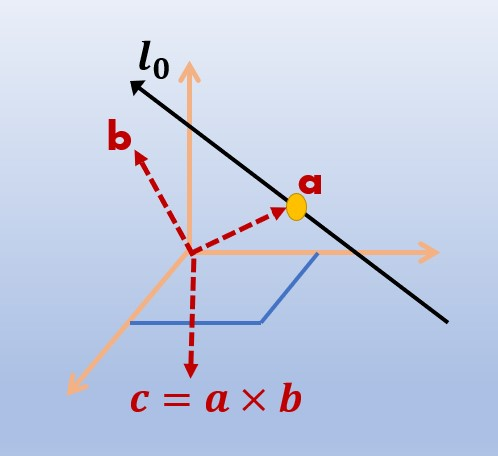
\includegraphics[width=\textwidth]{figures/plucker_coords.jpg}
		\end{column}
		\label{fig:plucker}
	\end{columns}
\end{frame}


\subsection{Displacement \& Twist}
\begin{frame}
	\frametitle{Screws and Pl{\"u}cker Coordinates}
	%
	\begin{block}{Screw axis and Pl{\"u}cker Coordinates}
		\begin{align}
			b_1 &= s_1, \quad b_2 = s_2, \quad b_3 = s_3; \\
			c_1 &= s_4 - p \cdot s_1, \quad c_2 = s_5-p\cdot s_2, \quad c_3 = s_6 - p\cdot s_3.
		\end{align}
	\end{block}
	%
	\begin{block}{Pitch in Pl{\"u}cker Coordinates}
		\begin{align}
			p &= \dfrac{s_1 \, s_4 + s_2 \, s_5 + s_3 \, s_6}{{s_1^2 + s_2^2 + s_3^2}}, \\
			\mid s \mid &= \sqrt{s_1^2 + s_2^2 + s_3^2} \quad \text{if } p \neq \infty, \\
			\mid s \mid &= \sqrt{s_4^2 + s_5^2 + s_6^2} \quad \text{if } p = \infty
		\end{align}
	\end{block}
\end{frame}


\begin{frame}
	\frametitle{Pitch and Magnitude of the screw}	
	\begin{block}{Pl{\"u}cker Coordinates' Direction Cosines}
		Suppose that 
		%\begin{align}
		$h = \sqrt{b_1^2+b_2^2+b_3^2}$.
		%\end{align}
		Then $(\bm{b}/h, \bm{c}/h)$ are respectively the direction cosines of the line, $l_0$ and its moment.
	\end{block}
	%
	\begin{block}{ Homogeneous Coordinates!}
		\textcolor{blue}{Pl{\"u}cker Coordinates} give six unit parameters of a point on a line. Pl{\"u}cker Coordinates are in \textcolor{red}{homogeneous coordinates}!
	\end{block}
\end{frame}

\begin{frame}
	\frametitle{Twist About a Screw (Axis)}
		%
		\begin{block}{Twist}
			A body's \textcolor{purple}{twist} about 
			s \textcolor{magenta}{screw} is a \textcolor{red}{uniform (infinitesimal) rotation} about the screw \textcolor{blue}{followed by a uniform (infinitesimal) translation} about an \textcolor{cyan}{axis parallel to the screw}, through \textcolor{magenta}{a distance that is the product of the pitch and the circular measure of rotation}.
		\end{block}	
		%
		\begin{block}{Twist}
			A \textcolor{purple}{twist} requires six 
			s \textcolor{magenta}{algebraic quantities} for its  \textcolor{red}{complete specification}:  \textcolor{blue}{five ($\{t_i\}_{i=1}^5$) specify the screw}, the \textcolor{cyan}{sixth (or its amplitude)} specifies the \textcolor{light-blue}{screw's rotaty angle}, $t_6$.
		\end{block}	
\end{frame}

\begin{frame}
	\frametitle{Twist in Pl{\"u}cker Coordinates}
	%
			\begin{definition}[Twist Coordinates]
				A six-vector, $\bm{t}$, related to the Pl{\"u}cker coordinates  parameterize a twist vector i.e. $\bm{t}=\left[(t_1, t_2, t_3), (t_4, t_5, t_6)\right]$ or $\bm{t}=\left(\bm{\omega}, \bm{v}\right)$, where $\bm{\omega}=(t_1, t_2, t_3)$ and $\bm{v}=(t_4, t_5, t_6)$.
			\end{definition}
	%
	\begin{block}{Pl{\"u}cker Coordinates of a Twist}
		\begin{align}
			b_1 &= t_1, \quad b_2 = t_2, \quad b_3 = t_3 \\
			c_1 &= t_4 - p \cdot s_1, \quad c_2 = t_5-p\cdot s_2, \quad c_3 = t_6 - p\cdot s_3.
		\end{align}
	%
\end{block}
\end{frame}

\begin{frame}
	\frametitle{Twists in Pl{\"u}cker Coordinates}
	%
	\begin{block}{Pitch of the Twist}
		$p_t = \dfrac{t_1\,t_4 + t_2 \, t_5 + t_3\,t_6}{t_1^2+t_2^2+t_3^2}=\dfrac{\bm{\omega}\cdot \bm{v}}{\bm{\omega}\cdot \bm{\omega}}$.
	\end{block}
	%
	\begin{block}{Pitch of the Twist}
		Expressed as a ratio of the \textcolor{magenta}{magnitude of the velocity of a point on the twist axis} to the \textcolor{green}{magnitude of the angular velocity} about the twist axis. 
	\end{block}	
	%
	\begin{block}{Translation Distance}
		$d_t = t_6 \times p_t$.  The sign expresses the rotation's direction.
	\end{block}	
\end{frame}


\begin{frame}
	\frametitle{Twists and Fixed Movements}
	\begin{block}{Pure Rotation}
		Let pitch be \textcolor{light-blue}{zero}. That which results is but \textcolor{red}{pure rotation}.
	\end{block}
	
	\begin{block}{Pure Translation}
		Let pitch be \textcolor{magenta}{infinite}. That which results \textcolor{red}{cannot be a finite twist}, \textcolor{cyan}{except the amplitude be zero}, whereupon the \textcolor{brown}{twist becomes a pure translation parallel to the screw}.
	\end{block}
\end{frame}

%
\begin{frame}
	\frametitle{Curvilinear Displacement: Serret-Frenet Frame}
	\begin{columns}[]
		\begin{column}{.5\linewidth}
			\centering
			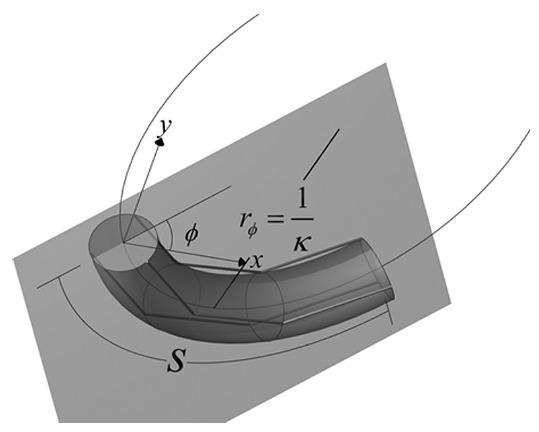
\includegraphics[width=\textwidth]{figures/multi_sec_manip.jpg}
		\end{column}
		\begin{column}{.68\linewidth}
			\centering
			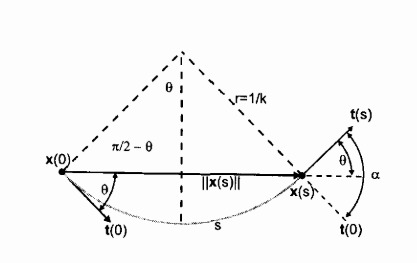
\includegraphics[width=\textwidth]{figures/serret.jpg}
		\end{column}
	\end{columns}
	\footnotesize{Elephant Trunk Multi-sectional Continuum Model (left), and its Representation in the Serret-Frenet Frame.}
\end{frame}
\begin{frame}
	\frametitle{Pl{\"u}cker Coordinates Example}
	\begin{block}{Chasles' Theorem Applied to The Serret-Frenet Frame}
		Consider a spatial curve $\bm{S}$ on the elephant continuum trunk shown earlier. Suppose $\bm{S}$ is parameterized by its arc length $\bm{s} \in [0, 1]$. 
		For a point $\bm{x}=\left[x, y, z\right]^T$ on $\bm{S}$, the unit tangent vector at $s$ is $\bm{t}(s)=\bm{dx}/\bm{ds}$.
	\end{block}
	%	
	\begin{block}{Differential Kinematics and The Serret-Frenet Frame}
		 Denote by $\bm{n}$ the principal normal to $\bm{S}$ at $\bm{n}$; then we must have $\bm{b}=\bm{t}\times \bm{n}$ as the binormal. We say $(\bm{b},\bm{n})$ is the Pl{\"u}cker coordinate of the tangent $\bm{t}$.
	\end{block}
\end{frame}

\subsection{Force \& Wrench}
\begin{frame}
	\frametitle{Force}
	%	
	\begin{block}{Force}
		Net \textcolor{blue}{force} exerted on a body, 
		$\textcolor{red}{\bm{F}} = (f_x, f_y, f_z)$.
	\end{block}
	\begin{block}{Couple of Force}
		Suppose that $\bm{F}$ acts along a corkscrew axis. The resulting motion when $\bm{F}$ makes an infinitesimal rotation about its screw axis  is called its \textcolor{red}{couple}, $\mathfrak{C} = (c_x, c_y, c_z)$.
	\end{block}
	%	
\end{frame}

\begin{frame}
	\frametitle{Complete Wrench on a Screw}
	%	
	\begin{block}{Wrench}		
		A \textcolor{purple}{wrench} requires six 
		s \textcolor{magenta}{algebraic quantities} for its  \textcolor{red}{complete specification}:  \textcolor{blue}{five ($\{w_i\}_{i=1}^5$) specify the screw}, the \textcolor{cyan}{sixth (or its intensity)}, $w_6$, specifies the \textcolor{light-blue}{force's magnitude}.
	\end{block}
	%		
	\begin{block}{Couple's Moment}		
		The moment of the \textcolor{purple}{couple} is the product of the \textcolor{magenta}{intensity of the wrench} and the \textcolor{red}{ and the screw's pitch} i.e. $\alpha(\mathfrak{C}) = w_6 \times p_w$.
	\end{block}
	%	
\end{frame}

\begin{frame}
	\frametitle{Wrench on a Screw}
	%	
	\begin{block}{Wrench}
		Simple Definition: A \textcolor{brown}{force} and a \textcolor{cyan}{couple} both acting in a plane perpendicular to the force.
	\end{block}
	%
	\begin{definition}[Complete Definition]		
		The \textcolor{brown}{resultant canonical system of forces} acting on a rigid body, \textcolor{light-blue}{reduced to a resultant force on a point}, and acting along the \textcolor{red}{resultant couple} that is \textcolor{cyan}{perpendicular to the plane} in which the force acts is called \textcolor{blue}{the wrench}.
	\end{definition}
	%	
\end{frame}

\begin{frame}
	\frametitle{Wrench in Pl{\"u}cker Coordinates}
	%
	\begin{definition}[Wrench Coordinates]
		A six-vector, $\bm{w}$, related to the Pl{\"u}cker coordinates  parameterize a wrench vector i.e. $\bm{w}=\left[(w_1, w_2, w_3), (w_4, w_5, w_6)\right]$ or $\bm{w}=\left(\bm{f}, \bm{m}\right)$, where $\bm{f}=(w_1, w_2, w_3)$ and $\bm{m}=(w_4, w_5, w_6)$.
	\end{definition}
	%
	\begin{block}{Pl{\"u}cker Coordinates of a Wrench}
		\begin{align}
			b_1 &= w_1, \quad b_2 = w_2, \quad b_3 = w_3 \\
			c_1 &= w_4 - p \cdot s_1, \quad c_2 = w_5-p\cdot s_2, \quad c_3 = t_6 - p\cdot w_3.
		\end{align}
		%
	\end{block}
\end{frame}

\begin{frame}
	\frametitle{Wrench in Pl{\"u}cker Coordinates}
	%
	\begin{block}{Pitch of the Wrench}
		$p_t = \dfrac{w_1\,w_4 + w_2 \, w_5 + w_3\,w_6}{w_1^2+w_2^2+w_3^2}=\dfrac{\bm{f}\cdot \bm{m}}{\bm{f}\cdot \bm{f}}$.
	\end{block}
	%
	\begin{block}{Pitch of the Wrench}
		Expressed as a ratio of the \textcolor{magenta}{moment applied about a point on the axis} to the \textcolor{light-blue}{magnitude of the force applied}  along the wrench axis. 
	\end{block}	
	%
	\begin{block}{Wrench's Magnitude}
		$\|f\| = \sqrt{w_1^2 + w_2^2 + w_3^2}$ if $p_w = 0$ else $\|m\| = \sqrt{w_4^2 + w_5^2 + w_6^2}$ if $p_w = \infty$.
	\end{block}	
\end{frame}

\begin{frame}
	\frametitle{Wrenches and Fixed Movements}
%	\begin{block}{Pitch of a Wrench, $p_w$}
%		Acts along a (corkscrew) axis,  $p_w\bm{F}=\mathfrak{C}$.
%	\end{block}
	%
	\begin{block}{Pure Force}
		Let pitch be \textcolor{light-blue}{zero}. That which results is \textcolor{red}{pure force} along its screw axis.
	\end{block}
	
	\begin{block}{Pure Couple}
		Let pitch be \textcolor{magenta}{infinite}. That which results \textcolor{red}{cannot be a finite wrench}, \textcolor{cyan}{except the intensity be zero}, whereupon the \textcolor{brown}{wrench becomes a pure couple in a plane that is perpendicular to the screw}.
	\end{block}
\end{frame}


\begin{frame}
	\frametitle{Statics and Instantaneous Kinematics}
	%
	\begin{block}{Statics and kinematics}
		\begin{center}
			\begin{tabular}{||c | c||} 
				\hline
				\textbf{Statics} & \textbf{Instantaneous Kinematics}  \\ %[0.5ex] 
				\hline\hline
				Force,  $\bm{F}$ about $n$. & Infinitesimal rotation, $\bm{\omega}$ \\ 
				\hline
				Couple, $\mathfrak{C}$: [$\bm{F}$] $\times$ [$\ell$] & Infinitesimal translation, $\bm{t}$ \\
				\hline
				$p_w = \pm \mathfrak{C}/\bm{F}$ & Pitch of a Wrench, $\bm{w}$ \\
				\hline
				$\mid\bm{F} \mid$ & Intensity of Wrench \\
				\hline
			\end{tabular}
			\text{Dyname}: $(\bm{F}, \mathfrak{C})$. Credits: Pl{\"u}cker (1866), Routh (1892).
		\end{center}
	\end{block}
	
\end{frame}

\subsection{Screws in Pl{\"u}cker Coordinates}
\begin{frame}
	\frametitle{Pl{\"u}cker Coordinates Kinetics Quiz}
	%
	\begin{block}{Poinsot's Theorem Quiz on a  Force and its Moment}
		Suppose that a force $\bm{F}$  acts at the point $\bm{a}$ in the image of Frame \ref{fig:plucker}. What are the Pl{\"u}cker coordinates of the \textcolor{red}{line of force}?
	\end{block}
\end{frame}

\note{
	\begin{frame}
		%
		\begin{block}{Poinsot's Theorem Quiz on a  Force and its Moment}
			Imagine that a force $\bm{F}$ is acting at the point $\bm{a}$ in the image of Frame \ref{fig:plucker}. Suppose that $\bm{\tau}$ is torque acting along the normal to point $\bm{a}$.  Then $(\bm{f,\tau})$ are the Pl{\"u}cker  coordinates of the \textcolor{red}{line of force}.
		\end{block}
		%
		\begin{block}{Arithmetics on Screws}
			Scalar and vector arithmetic operations are valid on infinitesimal  screws e.g.
			\begin{align}
				c_1 \bm{s}_1 + c_2 \bm{s}_2 = 0 \text{ for } c_1, \, c_2 \neq 0 \text{ on screws } \bm{s}_1, \bm{s}_2.
			\end{align}
		\end{block}
	\end{frame}
}

\subsection{$\mathbb{R}^3$ Motions}

\begin{frame}
	\frametitle{Pl{\"u}cker Coordinates Kinetics Quiz}
	%
	\begin{block}{Poinsot's Theorem Quiz on a  Force and its Moment}
		Suppose that a force $\bm{F}$  acts at the point $\bm{a}$ in the image of Frame \ref{fig:plucker}. What are the Pl{\"u}cker coordinates of the \textcolor{red}{line of force}?
	\end{block}
\end{frame}

\begin{frame}
	\frametitle{Rigid Body Transformations}
	%
	\begin{block}{Translation of Point $\bm{q}$ between Two Frames}
		For a reference frame, $o_0 x_0 y_0$ and a moving coordinate frame, $o_1 x_1 y_1$, the translation of $\bm{q}$ is given as below:
	\end{block}
	\begin{columns}[]
		\begin{column}{.5\linewidth}
			\centering
			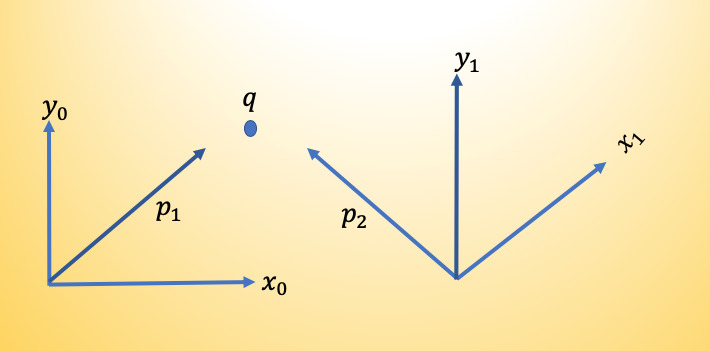
\includegraphics[width=\textwidth]{../Notes/figures/trans_coords.jpg}
		\end{column}
		\begin{column}{.5\linewidth}
			\begin{align}
				q^0 = \left( \begin{array}{c}
					q^0_x \\ q_y^0
				\end{array}
				\right), \quad
				%
				q^1 = \left( \begin{array}{c}
					q^1_x \\ q_y^1
				\end{array}
				\right) \nonumber
			\end{align}
		\end{column}
	\end{columns}
	%
	\begin{block}{Translation of Origin between Two Frames}
		\begin{align}
			o^0_1 = \left( \begin{array}{c}
				o^0_x \\ o^0_y
			\end{array}
			\right), \quad
			%
			o^1_0 = \left( \begin{array}{c}
				o^1_x \\ o^1_y
			\end{array}
			\right).
		\end{align}
	\end{block}
\end{frame}

\begin{frame}
	\frametitle{Rigid Body Transformations}
	%
	\begin{block}{Applications to Screws}
		Applies to Chasles' displacement theorem and Poinsot's force and couple transformations too.
	\end{block}
	%
	\begin{block}{Screw Transformations}
		\begin{align}
			\bm{t}^0_1 &= \left( \begin{array}{c}
				t^0_x \\  t^0_y %\\  t^0_z
			\end{array}
			\right),
			%
			\quad \bm{t}^1_1 = R(-\theta) q^0 \\
			%
		    \bm{t}^0_2 &= R(\theta) q^0, \quad \bm{t}^1_2 = \left( \begin{array}{c}
				t^1_x \\  t^1_y %\\  t^1_y
			\end{array}
			\right)
		\end{align}
		%
		where $\theta$ is the angle coordinate frame $o_1 x_1 y_1$ makes w.r.t $o_0 x_0 y_0$.
	\end{block}
\end{frame}

\begin{frame}
	\frametitle{Rotations in $\bb{R}^3$}
	%
	\begin{block}{Rotations in $\bb{R}^3$}
		Conventions: Bodies' \textcolor{blue}{orientations} are \textcolor{magenta}{measured along a corkscrew direction}, specified by a \textcolor{cyan}{local coordinate frame}. Thus, \textcolor{magenta}{relative orientation} is measured from the \textcolor{cyan}{local coordinate frame} to an \textcolor{magenta}{inertial coordinate frame}.
	\end{block}
	%
\end{frame}

\begin{frame}
	\frametitle{Direction Cosines}
	%
	\begin{columns}[]
		\begin{column}{.6\linewidth}
			\centering
			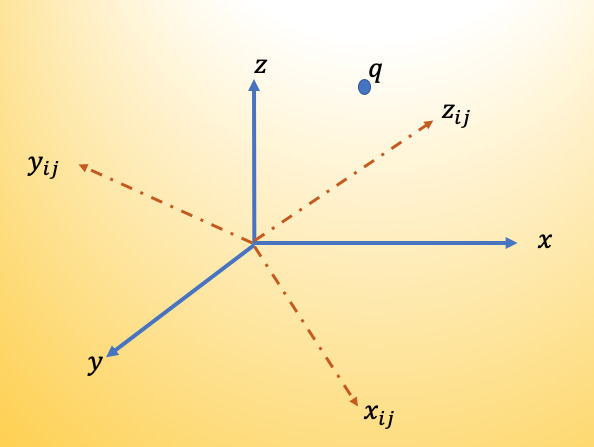
\includegraphics[width=\textwidth]{../Notes/figures/rotation_illus.jpg}
		\end{column}
		\begin{column}{.4\linewidth}
			\begin{block}{Conventions}
			 $I$: \textcolor{magenta}{Inertial frame}; $J$: \textcolor{cyan}{Body frame}.
				%
			$\bm{q}: (\bm{x}_{ij}, \bm{y}_{ij},\bm{z}_{ij}) \in \bb{R}^3$: coordinates of the \textcolor{purple}{principal axes} of $J$ relative to $I$.
			\end{block}
		\end{column}
	\end{columns}
\end{frame}


\begin{frame}
	\frametitle{Rotation Matrix from Direction Cosines}
	\begin{block}{Rotation as Composition of Projections Between Frames}
		\begin{align}
			R_{ij} = \begin{bmatrix}
				\bm{x}_{ij} \quad  \bm{y}_{ij} \quad \bm{z}_{ij}
			\end{bmatrix} = \begin{bmatrix}
				r_{11} &  r_{12} & r_{13} \\
				r_{21} & r_{22} &  r_{23} \\
				r_{31} & r_{32} &  r_{33}
			\end{bmatrix}.
			\label{eq:rotation_compoz}
		\end{align}
	\end{block}
	
	\begin{block}{Rotation Matrix as Unit Axes' Dot Products}
		\begin{align}
			R_{ij} = \begin{bmatrix}
				\bm{x}_j \cdot \bm{x}_i & \bm{y}_j \cdot \bm{x}_i & \bm{z}_j \cdot \bm{x}_i \\
				%
				\bm{x}_j \cdot \bm{y}_i & \bm{y}_j \cdot \bm{y}_i & \bm{z}_j \cdot \bm{y}_i \\
				%
				\bm{x}_j \cdot \bm{z}_i & \bm{y}_j \cdot \bm{z}_i & \bm{z}_j \cdot \bm{z}_i 
			\end{bmatrix}.
			\label{eq:direction_cosines}
		\end{align}
	\end{block}
\end{frame}

\begin{frame}
	\frametitle{Rotation Matrix from Direction Cosines}
	\begin{block}{Rotation Matrices are Direction Cosines!}
		$\bm{x}_j \cdot \bm{x}_i = \cos(\measuredangle\left(\bm{x}_j, \bm{x}_i\right)), \quad 	\bm{y}_j \cdot \bm{x}_i = \cos(\measuredangle\left(\bm{y}_j, \bm{x}_i\right)), \cdots$
		
		$\cdots, \bm{y}_j \cdot \bm{z}_i = \cos(\measuredangle\left(\bm{y}_j, \bm{z}_i\right)), \quad 	\bm{z}_j \cdot \bm{z}_i = \cos(\measuredangle\left(\bm{z}_j, \bm{z}_i\right)).$
	\end{block}
	
	\begin{block}{Properties of Rotation Matrices}
		Rows of $R_{ij}$ are the \textcolor{magenta}{unit vector} coordinates of $I$  in the frame $J$ so that 
		%
		\begin{align}
			R_{ij} =  R_{ji}^{-1} = R_{ji}^T.
		\end{align}
		%
		That is, the \textcolor{blue}{inverse of the rotation matrix is equal to its transpose}. 
	\end{block}
\end{frame}

\subsection{Special Orthogonal Properties}
\begin{frame}
	\frametitle{Special Orthogonal 3, SO(3)}
	\begin{block}{Orthogonal properties!}
			Observe: $\text{det }  \bm{R} = \bm{r}_1^T \cdot \left(\bm{r}_2 \times \bm{r}_3\right)$. In \textcolor{cyan}{corkscrew notation}, $\text{det }  \bm{R} = +1$ i.e. $\bm{r}_2 \times \bm{r}_3 = \bm{r}_1$ so that $\text{det }  \bm{R} = \bm{r}_1^T \cdot \bm{r}_1 = +1$. A matrix that satisfies the above property is said to \textcolor{light-blue}{possess a special orthogonal 3, denoted SO(3),  property}.
	\end{block}
	
	\begin{block}{SO(n) Property}
		Special orthogonal means $\text{det } \bm{R} = + 1$. The set of all SO matrices in $\bb{R}^{n\times n}$ is 
		%
		\begin{align}
			\text{SO(n)} = \{\bm{R}\in \bb{R}^{n\times n}: \bm{R}\cdot \bm{R}^T = \bm{I}, \text{det }\bm{R} = + 1\}.
		\end{align}
	\end{block}
\end{frame}

\begin{frame}
	\frametitle{Rotations on Vectors}
	\begin{columns}[]
		\begin{column}{.85\linewidth}
			\begin{block}{Rotating a Vector}
				Suppose that a point $p_j$ is on a frame $J$, then the vector that connects a point $q_j$ in the frame $J$ to $p_j$ is $v_j = q_j - p_j$. Now, the rotation matrix's action on $v_j$ is
				%
				\begin{align}
					\bm{R}_{ij}(v_j) := \bm{R}_{ij} q_j - \bm{R}_{ij} p_j = q_i - p_i = v_i.
				\end{align}
			\end{block}
		\end{column}
	\end{columns}
\end{frame}


\begin{frame}
	\frametitle{Planar Rotations}
	\begin{columns}[]
		\begin{column}{.5\linewidth}
			\begin{block}{Planar Rotations}
				Let the angle of rotation between the two coordinate frames be $\theta$. Then,
			\begin{align}
				R_1^0 = \left(\begin{array}{cc}
					x_1^0 \,\,| & y_1^0
				\end{array}\right)
			\end{align}
			\end{block}
		\end{column}
		\begin{column}{.5\linewidth}
			\centering
			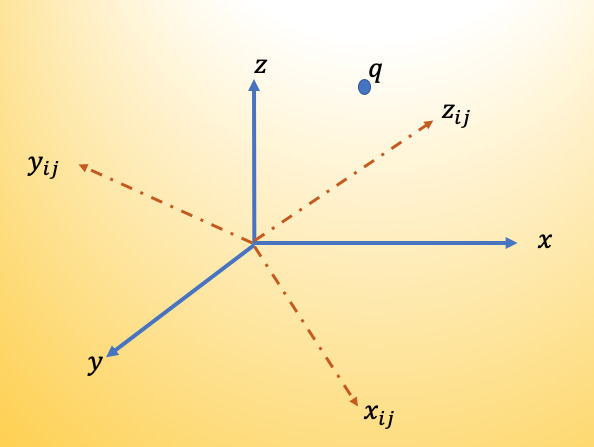
\includegraphics[width=\textwidth]{../Notes/figures/rotation_illus.jpg}
		\end{column}
	\end{columns}
	
	\begin{columns}[]
		\begin{column}{.5\linewidth}
			\begin{block}{Planar Rotations}
				It follows that
				\begin{align}
					R = \left(\begin{array}{cc}
						\cos \alpha & -\sin \alpha \\ \sin \alpha &  \cos \alpha
					\end{array}\right)
				\end{align}
			\end{block}
		\end{column}
		\begin{column}{.5\linewidth}
			\centering
			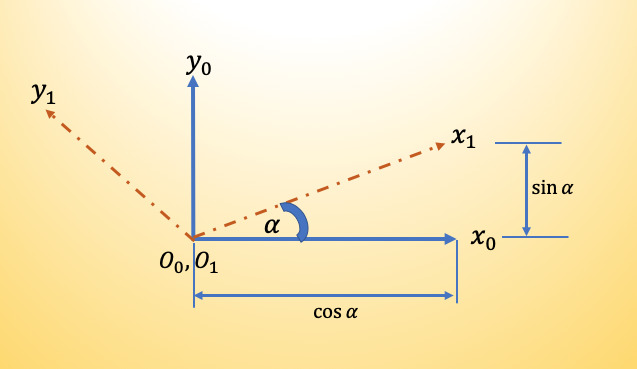
\includegraphics[width=\textwidth]{../Notes/figures/planar_rot.jpg}
		\end{column}
	\end{columns}
\end{frame}


\begin{frame}
	\frametitle{Planar Rotations}
			\begin{block}{Planar Rotations via Direction Cosines}
				\begin{align}
					R_1^0 &= \begin{bmatrix}
						\bm{x}_0 \cdot \bm{x}_1 & \bm{y}_1 \cdot \bm{x}_0 \\
						%
						\bm{x}_0 \cdot \bm{y}_1 & \bm{y}_1 \cdot \bm{y}_0
					\end{bmatrix} =  \begin{bmatrix}
					cos \alpha &  -cos(\pi/2 - \alpha) \\
					%
					cos(\pi/2 - \alpha) & cos \alpha
				\end{bmatrix} \nonumber \\
			%
		&=  \begin{bmatrix}
		cos \alpha &   - \sin \alpha  \\
		%
		\sin \alpha  & cos \alpha
	\end{bmatrix}.
				\end{align}
			\end{block}
		\footnotesize{Projection of $y_1$ on $x_0$ is negative because of our adopted right-handed frame.}
\end{frame}

\subsection{Composition of Rotations}
\begin{frame}
	\frametitle{Composition of Rotations}
			\begin{block}{Rotations Composition}
				Let the \textcolor{cyan}{relative orientation} of a frame $K$  to a frame $J$ be $\bm{R}_{jk}$, and let frame $J$'s  \textcolor{cyan}{relative orientation} to frame $I$ be $\bm{R}_{ij}$, then the \textcolor{cyan}{relative orientation} of frame $K$  w.r.t $I$ is 
				%
				\begin{align}
					\bm{R}_{ik} = \bm{R}_{ij} \cdot \bm{R}_{jk}.
				\end{align} 
			\end{block}
		
		\begin{block}{Rotations Composition}
			Equivalent to \textcolor{brown}{rotating $J$ relative to frame $I$ according to $\bm{R}_{ij}$}; then \textcolor{magenta}{aligning frame $J$  to $K$}, we \textcolor{light-blue}{rotate $K$ relative to $I$ according to $\bm{R}_{jk}$}. This frame relative to which rotation occurs is termed the \textcolor{light-red}{current frame}. 
		\end{block}
\end{frame}


\begin{frame}
	\frametitle{Composition of Rotations About A Current Axis}
	\begin{block}{Composition of Rotations About A Current Axis}
		%
		\centering
		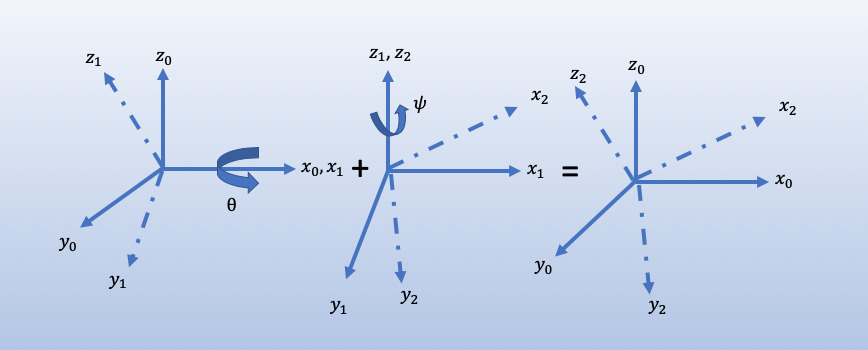
\includegraphics[width=1\textwidth]{../Notes/figures/compoz.jpg}
	\end{block}
\end{frame} 

\begin{frame}
	\frametitle{Composition of Rotations About A Current Axis}
	\begin{block}{Compositions}
		\begin{align}
			\bm{R} &= \bm{R}_{x, \theta} \bm{R}_{z, \psi} 
			%
			= \left(\begin{array}{ccc}
				1 & 0 & 0 \\
				0 & c_\theta & -s_\theta \\
				0 & s_\theta & c_\theta
			\end{array}\right) 
			%
			\cdot
			%
			\left(\begin{array}{ccc}
				c_\psi & -s_\psi & 0 \\
				s_\psi & c_\psi & 0 \\
				0 & 0 & 1
			\end{array}\right) \\
			%
			\bm{R} &= \left(\begin{array}{ccc}
				c_\psi & -s_\psi & 0 \\
				0 & c_\theta c_\psi &  -s_\theta \\
				s_\theta s_\psi & s_\theta c_\psi & c_\theta 
			\end{array}\right)
		\end{align}
		%
		\footnotesize{Notice how the order of multiplication is carried out, owing to the axis about which we are making the transformation.} 
	\end{block}
\end{frame} 

\begin{frame}
	\frametitle{Composition of Rotations About A Current Axis}
	\begin{block}{Skew Symmetry Operations}
		%
		What happens when the \textcolor{red}{order of multiplication is reversed}?
	\end{block}
	
%	\begin{block}{Skew Symmetry}
%		%
%		Turns out \textcolor{light-blue}{going from rotations about a current frame} to a \textcolor{blue}{fixed axis} and \textcolor{brown}{rotations from a fixed axis} to a \textcolor{light-red}{current frame} is equivalent to \textcolor{purple}{skew-symmetric operations on matrices} i.e. 
%		\begin{align}
%			\bm{R}_{x, \theta} \bm{R}_{z, \psi}  =  \left(\bm{R}_{z, \psi} \bm{R}_{x, \theta}\right)^\wedge
%		\end{align}
%	\end{block}
\end{frame} 


\begin{frame}
	\frametitle{Composition of Rotations}
	\begin{block}{Skew Symmetric Matrix}
		%
		\begin{align}
			(S)^\wedge = \left(\begin{array}{ccc}
				0 & -s_z & s_y \\
				s_z & 0 & -s_x \\
				-s_y & s_x & 0 
			\end{array}\right)
		\end{align}
	\end{block}

\begin{block}{Skew Symmetric Matrix}
%
Observe $s_{ij} = -s_{ji}$ for $i\neq j$ and $s_ii=0$
\end{block}
\end{frame}


\begin{frame}
	\frametitle{Composition of Rotations}
			\begin{block}{Pre-multiplication of Rotations}
				%
				A \textcolor{cyan}{rotation} about \textcolor{brown}{a fixed axis} requires a \textcolor{light-blue}{pre-multiplication}.
			\end{block}
		
		\begin{block}{Post-multiplication of Rotations}
			%
			A \textcolor{cyan}{rotation} about \textcolor{brown}{a current axis} necessitates a \textcolor{light-blue}{post-multiplication}.
		\end{block}
\end{frame}



\begin{frame}
	\frametitle{Rotations' Composition}
	\begin{columns}[]
		\begin{column}{.65\linewidth}
			\begin{block}{Rotations Composition}
				Suppose all axes of the inertial frame are successively rotated by $\beta$  around $x_0, y_0, z_0$ respectively. What is the transformation? Verify that (1) $R_{e, \beta} = I$ where $e$ is the axes about which we are rotating and $\beta$ is the angle of rotation; (2) The composition of rotations about $\beta$ and $\alpha$ in a successive manner implies that $R_{z, \beta}, R_{z, \alpha} = R_{z, \beta + \alpha}$, and (3) ${(R_{z, \beta})}^{-1} = R_{z, -\beta}$. 
			\end{block}
		\end{column}
		\begin{column}{.45\linewidth}
			\centering
			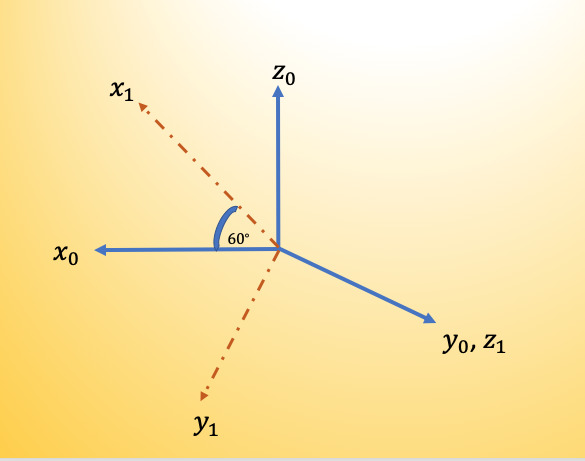
\includegraphics[width=\textwidth]{../Notes/figures/two_frames.jpg}
			\footnotesize{Relative orientation between two frames.}
		\end{column}
	\end{columns}
\end{frame}


\begin{frame}
	\frametitle{Euler Angles as Parameterization of Rotations}
	\begin{columns}[]
		\begin{column}{.95\linewidth}
			\centering
			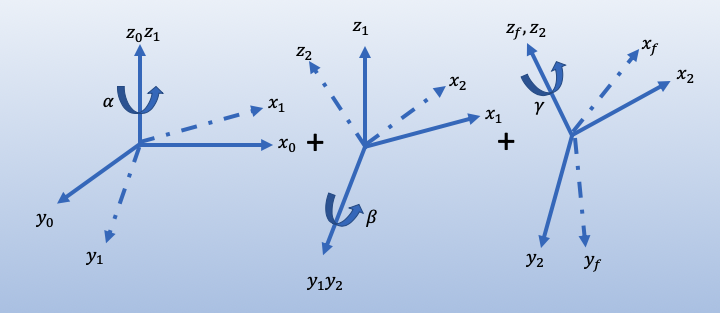
\includegraphics[width=\columnwidth]{../Notes/figures/zyz.png}
			\footnotesize{Relative orientation between two frames.}
		\end{column}
	\end{columns}
\end{frame}

\begin{frame}
	\frametitle{Euler Angles as Parameterization of Rotations}
			\begin{block}{Euler ($ZYZ$) Angles}
				\begin{align}
					\bm{R}_{ij}(\alpha, \beta, \gamma) &= \bm{R}_z(\alpha) \bm{R}_y(\beta) \bm{R}_z(\gamma) \\
					%
					& = \begin{bmatrix}
						c_\alpha & -s_\alpha & 0 \\
						%
						s_\alpha & c_\alpha & 0 \\
						%
						0 & 0 & 1
					\end{bmatrix}
					%
					\begin{bmatrix}
						c_\theta  & 0 & s_\theta\\
						%
						0  & 1 & 0 \\
						%
						-s_\theta  & 0 & c_\theta 
					\end{bmatrix} \nonumber \\
					%
					&= \begin{bmatrix}
						c_\alpha c_\beta c_\gamma - s_\alpha s_\gamma & -c_\alpha c_\beta s_\gamma - s_\alpha c_\gamma & c_\alpha s_\beta \\
						%
						s_\alpha c_\beta c_\gamma + c_\alpha s_\gamma & -s_\alpha c_\beta s_\gamma + c_\alpha c_\gamma  & s_\alpha s_\beta \\
						%
						-s_\beta c_\gamma & s_\beta s_\gamma & c_\beta
					\end{bmatrix} 
					\label{eq:zyz}
				\end{align} 
			\end{block}
\end{frame}

\begin{frame}
	\frametitle{Euler Angles as Parameterization of Rotations}
	\begin{block}{Euler ($ZYZ$) Angles. Case $\sin(\beta)>0$}
	\begin{subequations}
		\begin{align}
			\beta &= \arctan 2(r_{33}, \sqrt{1 - r_{33}^2})  \label{eq:euler_a}\\
			\alpha &= \arctan 2(r_{23}/\sin \beta, r_{13}/\sin \beta) \label{eq:euler_b} \\
			\gamma &= \arctan 2 (r_{32}/\sin \beta, -r_{31}/\sin \beta)
		\end{align}
		\label{eq:euler}
	\end{subequations}
	%
	\footnotesize{where $\arctan2(y, x)$ determines the quadrant of the angle based on the sign of $x$ and $y$}.
	\end{block}
\end{frame}

\begin{frame}
	\frametitle{Euler Angles as Parameterization of Rotations}
	\begin{block}{Euler ($ZYZ$) Angles. Case $\sin(\beta)<0$}
	\begin{subequations}
		\begin{align}
			\beta &=  \arctan2(r_{33}, -\sqrt{1 - r_{33}^2})  \label{eq:euler_neg_a}\\
			\alpha &= \arctan 2(-r_{23}/\sin \beta, -r_{13}/\sin \beta) \label{eq:euler_neg_b} \\
			\gamma &= \arctan 2 (-r_{32}/\sin \beta, r_{31}/\sin \beta)
		\end{align}
		\label{eq:euler_neg}
	\end{subequations}
		%
		\footnotesize{\textcolor{red}{Euler angles are not unique} owing to the sign of the angle about which the $y$ axis rotates!}
	\end{block}
\end{frame}


\begin{frame}
	\frametitle{Other Axes Parameterization of Rotations}
	\begin{block}{Fick ($ZYX$), Helmholtz ($YZX$) Angles.}
		 We could \textcolor{red}{permute the order of rotation} such as rotating successively about \textcolor{cyan}{different axes}. Examples include \textcolor{blue}{successive rotations about $ZYX$ axes for the Fick angles} and \textcolor{brown}{successive rotations about $YZX$ axes for Helmholtz angles}.
	\end{block}
	
	\begin{block}{Fick ($ZYX$) and Helmholtz ($YZX$) Angles.}
		These avoid \textcolor{blue}{Euler angle} \textcolor{red}{singularities} at $\bm{R} = \bm{I}$. This does not preclude \textcolor{red}{singularities at other configurations}.
	\end{block}
\end{frame}


\begin{frame}
	\frametitle{Fick angles and Yaw, Pitch, and Roll Axes}
	\begin{columns}[]
		\begin{column}{.45\linewidth}
			\begin{block}{Fick angles}
				Otherwise called the yaw, pitch, and roll angles. $\bm{R}_{ij}$ found by rotating about the $x-$axis  (roll), then the $y-$axis (pitch), and finally the $z-$axis -- all in the body frame. 
			\end{block}
		\end{column}
		\begin{column}{.55\linewidth}
			\centering
			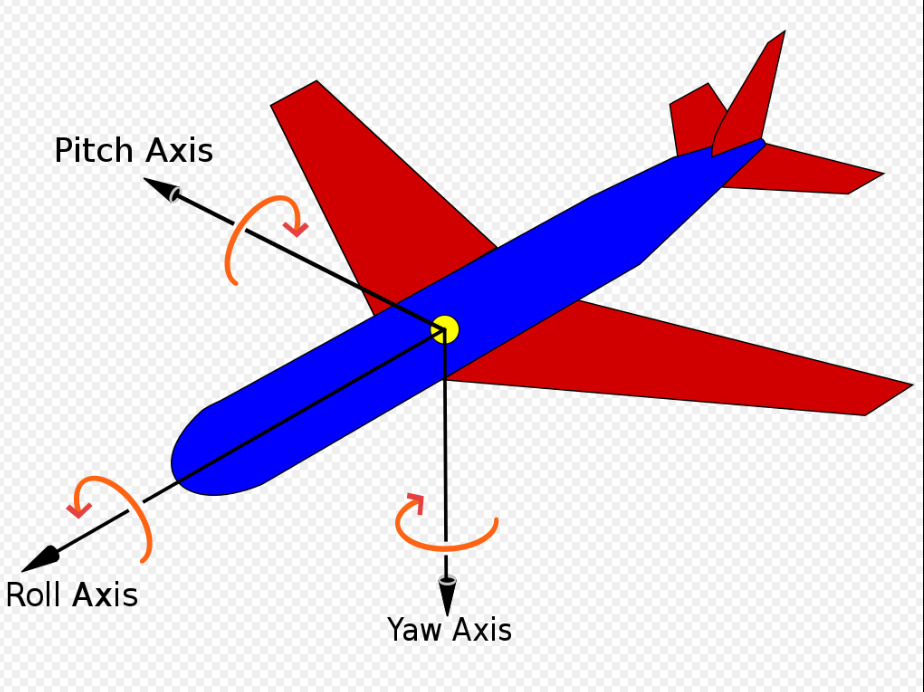
\includegraphics[width=\textwidth]{figures/yawpitchroll.jpg}
			\footnotesize{Aircraft Principal Axes in the right-hand frame. Courtesy of Wikimedia commons.}
		\end{column}
	\end{columns}
\end{frame}

\begin{frame}
	\begin{tcolorbox}[title=Summary of Parameterizations]
		Rotation matrices can be parameterized in one of many ways depending on our use case. The common examples of parameterizations are 
		%
		\begin{inparaenum}[\itshape (1)\upshape] \newline
			\item Axis-Angle representation; \newline
			\item Euler  angles ($ZYZ$) representation; \newline
			\item Fick  angles (\ie $ZYX$ or yaw, pitch and roll)  representation; \newline
			\item Helmholtz angles (or $YZX$) angles representation; and \newline
			\item Quaternions.
		\end{inparaenum}
		
	\end{tcolorbox}
\end{frame}